\documentclass[fontsize=10pt,a4paper]{scrartcl}

\usepackage{../../styles/myusepackages}
\usepackage{../../styles/mypythonstyle}
\usepackage{../../styles/myMCquestions}
\usepackage{../../styles/myframedenv}
%If graphics is listed before,some problems arise
\usepackage{graphicx}

\usepackage[english]{babel}
\usepackage[english,verbose]{layout}
\hypersetup{pdflang={es-ES}}

\newcommand{\academicyear}{2023-2024}
%%%%%%%%%%%%%%%%%%%%%%%%%%%%%%%%%%%%%%%%%%%%%%%%
%%%%%%%%%%%% TITLE
\title{Programing in Python\\ TEMA 6}
\usepackage{etoolbox}
\makeatletter
\providecommand{\subtitle}[1]{% add subtitle to \maketitle
  \apptocmd{\@title}{\par {\Huge #1 \par}}{}{}
}
\makeatother
\subtitle{\Large{Files}}
\author{Universidad Politécnica de Valencia}
\date{\academicyear{}}
%%%%%%%%%%%%%%%%%%%END TITLE%%%%%%%%%%%%%%%%%%%%%

\begin{document}
\maketitle
\tableofcontents


\chapter*{Prólogo}
\addcontentsline{toc}{chapter}{Prólogo}


¡Bienvenido a este libro de Python que te acompañará en el tema de programación durante el primer semestre de tus estudios universitarios!

Este libro se inspira en dos obras de código abierto:\textit{Python for Everybody} de Charles Severance \cite{severance2016python} y \textit{Think Python: How to Think Like a Computer Scientist} de Allen Downey \cite{downey2016thinkpython}. Estos libros han compartido su conocimiento bajo licencias de Creative Commons, formando la base del contenido de este libro.

La motivación para crear este libro surge de la necesidad de comprender sólidamente las pruebas (o el «testing») en la educación de programación. Creemos que las pruebas son una habilidad esencial en el mundo de la programación, pero sorprendentemente, este aspecto crucial a menudo se pasa por alto en los libros de programación para principiantes. Con el libro que tienes en tus manos, buscamos cambiar eso.

Integrar el «testing» en un curso de programación para principiantes no es fácil. Es por eso que utilizamos el innovador enfoque TILE \cite{10132188} «Test Informed Learning with Examples» o el Aprendizaje Informado por Pruebas con Ejemplos. El enfoque TILE se centra en integrar las pruebas de software en tu experiencia de programación introductoria de manera efectiva y placentera. TILE fue desarrollado con el generoso apoyo y financiamiento del proyecto Erasmus+ QPeD (número de contrato 2020-1-NL01-KA203-064626) y del proyecto ENACTEST (número de proyecto 101055874).

Con TILE, las pruebas se convierten en una parte integral de tu trayecto de programación desde el principio. Creemos firmemente que las pruebas no deben ser una idea secundaria, sino un aspecto esencial de tu proceso de codificación. Por eso te presentamos las pruebas desde el primer programa de ejemplo que encuentres.

Nuestro objetivo es dotarte del conocimiento y las habilidades para que te conviertas en un programador Python competente, armado con el poder de las pruebas para crear programas de alta calidad.

Así que, mientras te sumerges en el emocionante mundo de Python, recuerda que este libro está aquí para guiarte paso a paso en el dominio tanto de la programación como de las pruebas. Juntos, embarquémonos en este viaje mientras exploramos las maravillas de Python y el arte de las pruebas de software.

¡Feliz aprendizaje!

Tanja Vos
(tvos@dsic.upv.es)

\hypertarget{persistencia}{%
\section{Persistencia}\label{persistencia}}

\index{persistencia} \index{memoria secundaria}

Hasta ahora, hemos aprendido cómo escribir programas y comunicar
nuestras intenciones a la \emph{Unidad Central de Procesamiento}
utilizando ejecuciones condicionales, funciones, e iteraciones. Hemos
aprendido como crear y usar estructuras de datos en la \emph{Memoria
Principal}. La CPU y la memoria son los lugares donde nuestro software
funciona y se ejecuta. Es donde toda la \emph{inteligencia} ocurre.

Pero si recuerdas nuestras discusiones de arquitectura de hardware, una
vez que la corriente se interrumpe, cualquier cosa almacenada ya sea en
la CPU o en la memoria es eliminada. Así que hasta ahora nuestros
programas han sido sólo una diversión pasajera para aprender Python.

\begin{figure}
\centering
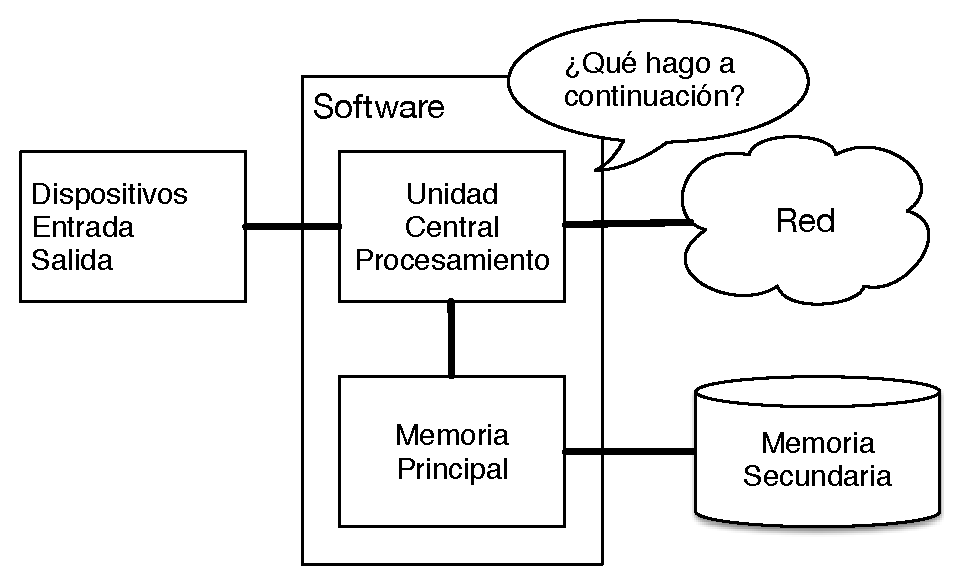
\includegraphics[width=0.6\textwidth]{images/arch.eps}
\caption{Memoria Secundaria}
\end{figure}

En este capítulo, vamos a comenzar a trabajar con \emph{Memoria
Secundaria} (o ficheros). La memoria secundaria no es eliminada cuando
apagamos una computadora. Incluso, en el caso de una memoria USB, los
datos que escribimos desde nuestros programas pueden ser retirados del
sistema y transportados a otro sistema.

Nos vamos a enfocar principalmente en leer y escribir ficheros como los
que creamos en un editor de texto. Más adelante veremos cómo trabajar
con ficheros de bases de datos, que son ficheros binarios diseñados
específicamente para ser leídos y escritos a través de software para
manejo de bases de datos.

\hypertarget{abrir-ficheros}{%
\section{Abrir ficheros}\label{abrir-ficheros}}

\index{fichero!abrir} \index{abrir función} \index{función!abrir}

Cuando queremos abrir o escribir un fichero (digamos, en el disco duro),
primero debemos \emph{abrir} el fichero. Al abrir el fichero nos
comunicamos con el sistema operativo, el cual sabe dónde están
almacenados los datos de cada fichero. Cuando abres un fichero, le estás
pidiendo al sistema operativo que encuentre el fichero por su nombre y
se asegure de que existe. En este ejemplo, abrimos el fichero
\emph{mbox.txt}, el cual debería estar almacenado en el mismo directorio
en que estás localizado cuando inicias Python. Puedes descargar este
fichero en Poliformat.

\begin{Verbatim}[frame=single]
>>> manejador_fichero = open('mbox.txt')
>>> print(manejador_fichero)
  <_io.TextIOWrapper name='mbox.txt' mode='r' encoding='cp1252'>
\end{Verbatim}

\index{manejador fichero}

Si el \pythoninline{open} es exitoso, el sistema operativo nos devuelve un
\emph{manejador de fichero}. El manejador de fichero no son los datos
contenidos en el fichero, sino un ``manejador'' \emph{(handler)} que
podemos usar para leer los datos. Obtendrás un manejador de fichero si
el fichero solicitado existe y si tienes los permisos apropiados para
leerlo.

\begin{figure}
\centering
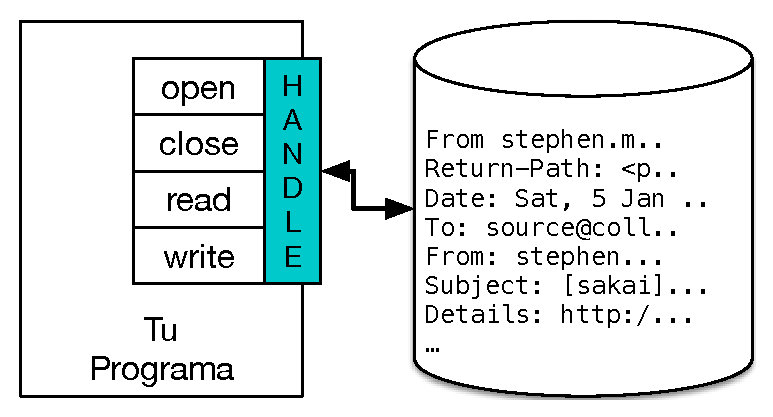
\includegraphics[width=0.6\textwidth]{images/handle.eps}
\caption{Un Manejador de fichero}
\end{figure}

Si el fichero no existe, \pythoninline{open} fallará con un mensaje de error y
no obtendrás un manejador para acceder al contenido del fichero:

\begin{Verbatim}[frame=single]
>>> manejador_fichero = open('stuff.txt')
Traceback (most recent call last):
File "<stdin>", line 1, in <module>
FileNotFoundError: [Errno 2] No such file or directory: 'stuff.txt'
\end{Verbatim}

Más adelante vamos a utilizar \pythoninline{try} y \pythoninline{except} para
controlar de mejor manera la situación donde tratamos de abrir un
fichero que no existe.

\hypertarget{ficheros-de-texto-y-luxedneas}{%
\section{Ficheros de texto y líneas}\label{ficheros-de-texto-y-luxedneas}}

Un fichero de texto puede ser considerado como una secuencia de líneas,
así como una cadena de Python puede ser considerada como una secuencia
de caracteres. Por ejemplo, este es un ejemplo de un fichero de texto
que registra la actividad de correos de varias personas en un equipo de
desarrollo de un proyecto de código abierto (open source):

\begin{Verbatim}[frame=single]
From stephen.marquard@uct.ac.za Sat Jan  5 09:14:16 2008
Return-Path: <postmaster@collab.sakaiproject.org>
Date: Sat, 5 Jan 2008 09:12:18 -0500
To: source@collab.sakaiproject.org
From: stephen.marquard@uct.ac.za
Subject: [sakai] svn commit: r39772 - content/branches/
Details: http://source.sakaiproject.org/viewsvn/?view=rev&rev=39772
...
\end{Verbatim}

El fichero completo de interacciones por correo está disponible en Poliformat con nombre \texttt{mbox.txt} y una versión reducida del fichero está disponible en
\texttt{mbox-short.txt}.

Esos ficheros están en un formato estándar para un fichero que contiene
múltiples mensajes de correo. Las líneas que comienzan con ``From''
separan los mensajes y las líneas que comienzan con ``From:'' son parte
de esos mensajes. Para más información acerca del formato mbox, consulta
\url{https://es.wikipedia.org/wiki/Mbox}.

Para separar el fichero en líneas, hay un carácter especial que
representa el ``final de una línea'' llamado \emph{salto de línea}.

\index{saltodelinea}

En Python, representamos el \emph{salto de línea} como una barra
invertida-n en las cadenas. Incluso aunque esto parezca dos caracteres,
realmente es un solo carácter. Cuando vemos la variable interactuando
con el intérprete, este nos muestra el \verb|\n| en la
cadena, pero cuando usamos \pythoninline{print} para mostrar la cadena, vemos
la cadena separada en dos líneas debido al salto de línea.

\begin{Verbatim}[frame=single]
>>> cosa = 'Hola\nMundo!'
>>> cosa
'Hola\nMundo!'
>>> print(cosa)
Hola
Mundo!
>>> cosa = 'X\nY'
>>> print(cosa)
X
Y
>>> len(cosa)
3
\end{Verbatim}

También puedes ver que el tamaño de la cadena
\verb|X\nY| es \emph{tres} caracteres debido a que el
separador de línea es un solo carácter.

Por tanto, cuando vemos las líneas en un fichero, necesitamos
\emph{imaginar} que ahí hay un carácter invisible llamado separador de
línea al final de cada línea, el cual marca el final de la misma.

De modo que el separador de línea separa los caracteres del fichero en
líneas.

\hypertarget{lectura-de-ficheros}{%
\section{Lectura de ficheros}\label{lectura-de-ficheros}}

\index{fichero!lectura} \index{contador}

Aunque el \emph{manejador de fichero} no contiene los datos de un
fichero, es bastante fácil utilizarlo en un bucle \pythoninline{for-in} para leer
a través del fichero y contar cada una de sus líneas:

\begin{python}[frame=single]
manejador_fichero = open('mbox-short.txt')
contador = 0
for linea in manejador_fichero:
    contador = contador + 1
print('Contador de líneas:', contador)
\end{python}

Podemos usar el manejador de ficheros como una secuencia en nuestro
bucle \pythoninline{for}. Nuestro bucle \pythoninline{for} simplemente cuenta el
número de líneas en el fichero y las imprime. La traducción aproximada
de ese bucle al español es, ``para cada línea en el fichero representado
por el manejador de fichero, suma uno a la variable \pythoninline{count}.''

La razón por la cual la función \pythoninline{open} no lee el fichero completo
es porque el fichero puede ser muy grande, incluso con muchos gigabytes
de datos. La sentencia \pythoninline{open} emplea la misma cantidad de tiempo
sin importar el tamaño del fichero. De hecho, es el bucle \pythoninline{for}
el que hace que los datos sean leídos desde el fichero.

Cuando el fichero es leído usando un bucle \pythoninline{for} de esta manera,
Python se encarga de dividir los datos del fichero en líneas separadas
utilizando el separador de línea. Python lee cada línea hasta el
separador e incluye el separador como el último carácter en la variable
\pythoninline{linea} para cada iteración del bucle \pythoninline{for}.

Debido a que el bucle \pythoninline{for} lee los datos línea a línea, éste
puede leer eficientemente y contar las líneas en ficheros muy grandes
sin quedarse sin memoria principal para almacenar los datos. El programa
previo puede contar las líneas de cualquier tamaño de fichero utilizando
poca memoria, puesto que cada línea es leída, contada, y después
descartada.

Si sabes que el fichero es relativamente pequeño comparado al tamaño de
tu memoria principal, puedes leer el fichero completo en una sola cadena
utilizando el método \pythoninline{read} en el manejador de ficheros.

\begin{Verbatim}[frame=single]
>>> manejador_fichero = open('mbox-short.txt')
>>> inp = manejador_fichero.read()
>>> print(len(inp))
94626
>>> print(inp[:20])
From stephen.marquar
\end{Verbatim}

En este ejemplo, el contenido completo (todos los 94626 caracteres) del
fichero \emph{mbox-short.txt} son leídos directamente en la variable
\pythoninline{inp}. Utilizamos el troceado de cadenas para imprimir los
primeros 20 caracteres de la cadena de datos almacenada en \pythoninline{inp}.

Cuando el fichero es leído de esta forma, todos los caracteres
incluyendo los saltos de línea son una cadena gigante en la variable
\pythoninline{inp}. Es una buena idea almacenar la salida de \pythoninline{read}
como una variable porque cada llamada a \pythoninline{read} vacía el contenido
por completo:

\begin{Verbatim}[frame=single]
>>> manejador = open('mbox-short.txt')
>>> print(len(manejador.read()))
94626
>>> print(len(manejador.read()))
0
\end{Verbatim}

Recuerda que esta forma de la función \pythoninline{open} solo debe ser
utilizada si los datos del fichero son apropiados para la memoria
principal del sistema. Si el fichero es muy grande para caber en la
memoria principal, deberías escribir tu programa para leer el fichero en
bloques utilizando un bucle \pythoninline{for} o \pythoninline{while}.

\hypertarget{buxfasqueda-a-travuxe9s-de-un-fichero}{%
\section{Búsqueda a través de un
fichero}\label{buxfasqueda-a-travuxe9s-de-un-fichero}}

Cuando buscas a través de los datos de un fichero, un patrón muy común
es leer el fichero, ignorar la mayoría de las líneas y solamente
procesar líneas que cumplan con una condición particular. Podemos
combinar el patrón de leer un fichero con métodos de cadenas para
construir mecanismos de búsqueda sencillos.

\index{filtro patron} \index{patron!filtro}

Por ejemplo, si queremos leer un fichero y solamente imprimir las líneas
que comienzan con el prefijo ``From:'', podríamos usar el método de
cadenas \emph{startswith} para seleccionar solo aquellas líneas con el
prefijo deseado:

%%\VerbatimInput{../code3/search1.py}
\begin{python}[frame=single]
man_f = open('mbox-short.txt')
contador = 0
for linea in man_f:
    if linea.startswith('From:'):
        print(linea)
\end{python}

Cuando este programa se ejecuta, obtenemos la siguiente salida:

\begin{Verbatim}[frame=single]
From: stephen.marquard@uct.ac.za

From: louis@media.berkeley.edu

From: zqian@umich.edu

From: rjlowe@iupui.edu
...
\end{Verbatim}

La salida parece correcta puesto que las líneas que estamos buscando son
aquellas que comienzan con ``From:'', pero ¿por qué estamos viendo las
líneas vacías extras? Esto es debido al carácter invisible \emph{salto
de línea}. Cada una de las líneas leídas termina con un salto de línea,
así que la sentencia \pythoninline{print} imprime la cadena almacenada en la
variable \pythoninline{linea}, la cual incluye ese salto de línea, y después
\pythoninline{print} agrega \emph{otro} salto de línea, resultando en el
efecto de doble salto de línea que observamos.

Podemos usar troceado de líneas para imprimir todos los caracteres
excepto el último, pero una forma más sencilla es usar el método
\pythoninline{rstrip}, el cual elimina los espacios en blanco del lado derecho
de una cadena, tal como:

%\VerbatimInput{../code3/search2.py}
\begin{python}[frame=single]
man_f = open('mbox-short.txt')
for linea in man_f:
    linea = linea.rstrip()
    if linea.startswith('From:'):
        print(linea)
\end{python}

Cuando este programa se ejecuta, obtenemos lo siguiente:

\begin{Verbatim}[frame=single]
From: stephen.marquard@uct.ac.za
From: louis@media.berkeley.edu
From: zqian@umich.edu
From: rjlowe@iupui.edu
From: zqian@umich.edu
From: rjlowe@iupui.edu
From: cwen@iupui.edu
...
\end{Verbatim}

A medida que tus programas de procesamiento de ficheros se vuelven más
complicados, quizá quieras estructurar tus bucles de búsqueda utilizando
\pythoninline{continue}. La idea básica de un bucle de búsqueda es que estás
buscando líneas ``interesantes'' e ignorando líneas ``no interesantes''.
Y cuando encontramos una línea interesante, hacemos algo con ella.

Podemos estructurar el bucle para seguir el patrón de ignorar las líneas
no interesantes así:

%\VerbatimInput{../code3/search3.py}
\begin{python}[frame=single]
man_f = open('mbox-short.txt')
for linea in man_f:
    linea = linea.rstrip()
    # Ignorar 'líneas que no nos interesan'
    if not linea.startswith('From:'):
        continue
    # Procesar la línea que nos 'interesa'
    print(linea)

\end{python}

La salida del programa es la misma. En Español, las líneas no
interesantes son aquellas que no comienzan con ``From:'', así que las
saltamos utilizando \pythoninline{continue}. En cambio las líneas
``interesantes'' (aquellas que comienzan con ``From:'') las procesamos.

Podemos usar el método de cadenas \pythoninline{find} para simular la función
de búsqueda de un editor de texto, que encuentra las líneas donde
aparece la cadena de búsqueda en alguna parte. Puesto que \pythoninline{find}
busca cualquier ocurrencia de una cadena dentro de otra y devuelve la
posición de esa cadena o -1 si la cadena no fue encontrada, podemos
escribir el siguiente bucle para mostrar las líneas que contienen la
cadena ``@uct.ac.za'' (es decir, los que vienen de la Universidad de
Cape Town en Sudáfrica):

%\VerbatimInput{../code3/search4.py}
\begin{python}[frame=single]
man_f = open('mbox-short.txt')
for linea in man_f:
    linea = linea.rstrip()
    if linea.find('@uct.ac.za') == -1: continue
    print(linea)
\end{python}

Lo cual produce la siguiente salida:

\begin{Verbatim}[frame=single]
From stephen.marquard@uct.ac.za Sat Jan  5 09:14:16 2008
X-Authentication-Warning: set sender to stephen.marquard@uct.ac.za using -f
From: stephen.marquard@uct.ac.za
Author: stephen.marquard@uct.ac.za
From david.horwitz@uct.ac.za Fri Jan  4 07:02:32 2008
X-Authentication-Warning: set sender to david.horwitz@uct.ac.za using -f
From: david.horwitz@uct.ac.za
Author: david.horwitz@uct.ac.za
...
\end{Verbatim}

Aquí utilizamos la forma contraída de la sentencia \pythoninline{if} donde
ponemos el \pythoninline{continue} en la misma línea que el \pythoninline{if}. Esta
forma contraída del \pythoninline{if} funciona de la misma manera que si el
\pythoninline{continue} estuviera en la siguiente línea e indentado.

\hypertarget{permitiendo-al-usuario-elegir-el-nombre-de-fichero}{%
\section{Permitiendo al usuario elegir el nombre de
fichero}\label{permitiendo-al-usuario-elegir-el-nombre-de-fichero}}

Definitivamente no queremos tener que editar nuestro código Python cada
vez que queremos procesar un fichero diferente. Sería más útil pedir al
usuario que introduzca el nombre del fichero cada vez que el programa se
ejecuta, de modo que pueda usar nuestro programa en diferentes ficheros
sin tener que cambiar el código.

Esto es sencillo de hacer leyendo el nombre de fichero del usuario
utilizando \pythoninline{input} como se muestra a continuación:

%\VerbatimInput{../code3/search6.py}
\begin{python}[frame=single]
nombre_f = input('Ingresa un nombre de un fichero: ')
man_f = open(nombre_f)
contador = 0
for linea in man_f:
    if linea.startswith('Subject:'):
        contador = contador + 1
print('Hay', contador, 'líneas de asunto (subject) en', nombre_f)
\end{python}

Leemos el nombre de fichero del usuario y lo guardamos en una variable
llamada \pythoninline{man_f} y abrimos el fichero. Ahora podemos ejecutar el programa repetidamente en diferentes ficheros.

\begin{Verbatim}[frame=single]
>>> %Run
  Ingresa un nombre de fichero: mbox.txt
  Hay 1797 líneas de asunto (subject) en mbox.txt
>>> %Run
  Ingresa un nombre de fichero: mbox-short.txt
  Hay 27 líneas de asunto (subject) en mbox-short.txt
\end{Verbatim}

Antes de mirar la siguiente sección, observa el programa anterior y
pregúntate a ti mismo, ``¿Qué error podría suceder aquí?'' o ``¿Qué
podría nuestro amigable usuario hacer que cause que nuestro pequeño
programa termine no exitosamente con un error, haciéndonos ver
no-muy-geniales ante los ojos de nuestros usuarios?''

\hypertarget{utilizando-try-except-y-open}{%
\section{\texorpdfstring{Utilizando try,\ except, y
open}{Utilizando try, except, y open}}\label{utilizando-try-except-y-open}}

Te dije que no miraras. Esta es tu última oportunidad.

¿Qué tal si nuestro usuario escribe algo que no es un nombre de fichero?

\begin{Verbatim}[frame=single]
>>> %Run
Ingresa un nombre de fichero: missing.txt
Traceback (most recent call last):
  File "search6.py", line 2, in <module>
    man_a = open(nfichero)
FileNotFoundError: [Errno 2] No such file or directory: 'missing.txt'
>>> %Run
Ingresa un nombre de fichero: na na boo boo
Traceback (most recent call last):
  File "search6.py", line 2, in <module>
    man_a = open(nfichero)
FileNotFoundError: [Errno 2] No such file or directory: 'na na boo boo'
\end{Verbatim}

No te rías. Los usuarios eventualmente harán cualquier cosa que puedan
para estropear tus programas, sea a propósito o sin intenciones
maliciosas. De hecho, una parte importante de cualquier equipo de
desarrollo de software es una persona o grupo llamado \emph{Quality
Assurance} (Control de Calidad) (o QA en inglés) cuyo trabajo es probar
las cosas más locas posibles en un intento de hacer fallar el software
que el programador ha creado.

\index{Control de Calidad} \index{QA}

El equipo de QA (Control de Calidad) es responsable de encontrar los
fallos en los programas antes de éstos sean entregados a los usuarios
finales, que podrían comprar nuestro software o pagar nuestro salario
por escribirlo. Así que el equipo de QA es el mejor amigo de un
programador.

\index{try sentencia} \index{sentencia!try} \index{abrir funcion}
\index{funcion!abrir} \index{excepcion!IOError} \index{IOError}

Ahora que vemos el defecto en el programa, podemos arreglarlo de forma
elegante utilizando la estructura \pythoninline{try}/\pythoninline{except}.
Necesitamos asumir que la llamada a \pythoninline{open} podría fallar y
agregar código de recuperación para ese fallo, así:

%\VerbatimInput{../code3/search7.py}
\begin{python}[frame=single]
nombre_f = input('Ingresa un nombre de archivo: ')
try:
    man_f = open(nombre_f)
except:
    print('No se puede abrir el archivo:', nombre_f)
    exit()
contador = 0
for linea in man_f:
    if linea.startswith('Subject:'):
        contador = contador + 1
print('Hay', contador, 'líneas de asunto (subject) en', nombre_f)
\end{python}

La función \pythoninline{exit} termina el programa. Es una función que
llamamos que nunca retorna. Ahora cuando nuestro usuario (o el equipo de
QA) introduzca algo sin sentido o un nombre de fichero incorrecto, vamos
a ``capturarlo'' y recuperarnos de forma elegante:

\begin{Verbatim}[frame=single]
>>> %Run
Ingresa un nombre de fichero: mbox.txt
Hay 1797 líneas de asunto (subject) en mbox.txt
>>> %Run
Ingresa un nombre de fichero: na na boo boo
No se puede abrir el fichero: na na boo boo
\end{Verbatim}

\index{Pythonic}
Proteger la llamada a \pythoninline{open} es un buen ejemplo del uso correcto
de \pythoninline{try} y \pythoninline{except} en un programa de Python. Utilizamos
el término ``Pythónico'' cuando estamos haciendo algo según el ``estilo
de Python''. Podríamos decir que el ejemplo anterior es una forma
Pythónica de abrir un fichero.

Una vez que estés más familiarizado con Python, puedes intercambiar
opiniones con otros programadores de Python para decidir cuál de entre
dos soluciones equivalentes a un problema es ``más Pythónica''. El
objetivo de ser ``más Pythónico'' engloba la noción de que programar es
en parte ingeniería y en parte arte. No siempre estamos interesados sólo
en hacer que algo funcione, también queremos que nuestra solución sea
elegante y que sea apreciada como elegante por nuestros compañeros.

\hypertarget{escritura-de-ficheros}{%
\section{Escritura de ficheros}\label{escritura-de-ficheros}}

\index{fichero!escritura}

Para escribir en un fichero, tienes que abrirlo en modo ``w'' (de
\pythoninline{write}, escritura) como segundo parámetro:

\begin{Verbatim}[frame=single]
>>> fsal = open('salida.txt', 'w')
>>> print(fsal)
<_io.TextIOWrapper name='salida.txt' mode='w' encoding='cp1252'>
\end{Verbatim}

Si el fichero ya existía previamente, abrirlo en modo de escritura
causará que se borre todo el contenido del fichero, así que ¡ten
cuidado! Si el fichero no existe, un nuevo fichero es creado.

El método \pythoninline{write} del manejador de ficheros escribe datos dentro
del fichero, devolviendo el número de caracteres escritos. El modo de
escritura por defecto es texto para escribir (y leer) cadenas.

\begin{Verbatim}[frame=single]
>>> linea1 = "Aquí está el zarzo,\n"
>>> fsal.write(linea1)
20
\end{Verbatim}

\index{saltodelinea}

El manejador de fichero mantiene un seguimiento de dónde está, así que
si llamas a \pythoninline{write} de nuevo, éste agrega los nuevos datos al
final.

Debemos asegurarnos de gestionar los finales de las líneas conforme vamos escribiendo en el fichero, insertando explícitamente el carácter
de salto de línea cuando queremos finalizar una línea. La sentencia
\pythoninline{print} agrega un salto de línea automáticamente, pero el método
\pythoninline{write} no lo agrega de forma automática.

\begin{Verbatim}[frame=single]
>>> linea2 = 'el símbolo de nuestra tierra.\n'
>>> fsal.write(linea2)
30
\end{Verbatim}

Cuando terminas de escribir, tienes que cerrar el fichero para
asegurarte que la última parte de los datos es escrita físicamente en el
disco duro, de modo que no se pierdan los datos si la corriente
eléctrica se interrumpe.

\begin{Verbatim}[frame=single]
>>> fsal.close()
\end{Verbatim}

Podríamos cerrar los ficheros abiertos para lectura también, pero
podemos ser menos rigurosos si sólo estamos abriendo unos pocos ficheros
puesto que Python se asegura de que todos los ficheros abiertos sean
cerrados cuando termina el programa. En cambio, cuando estamos
escribiendo ficheros debemos cerrarlos de forma explícita para no dejar
nada al azar.

\index{cerrar metodo} \index{metodo!cerrar}

\hypertarget{depuraciuxf3n}{%
\section{Depuración}\label{depuraciuxf3n}}

\index{depuracion} \index{espacioenblanco}

Cuando estás leyendo y escribiendo ficheros, puedes tener problemas con
los espacios en blanco. Esos errores pueden ser difíciles de depurar
debido a que los espacios, tabuladores, y saltos de línea son invisibles
normalmente:

\begin{Verbatim}[frame=single]
>>> s = '1 2\t 3\n 4'
>>> print(s)
1 2  3
 4
\end{Verbatim}

\index{repr funcion} \index{funcion!repr} \index{cadena representacion}

La función nativa \pythoninline{repr} puede ayudarte. Recibe cualquier objeto
como argumento y devuelve una representación del objeto como una cadena.
En el caso de las cadenas, representa los espacios en blanco con
secuencias de barras invertidas:

\begin{Verbatim}[frame=single]
>>> print(repr(s))
'1 2\t 3\n 4'
\end{Verbatim}

Esto puede ser útil para depurar.

Otro problema que podrías tener es que diferentes sistemas usan
diferentes caracteres para indicar el final de una línea. Algunos
sistemas usan un salto de línea, representado como
\verb|\n|. Otros usan un carácter de retorno,
representado con \verb|\r|. Otros usan ambos. Si mueves
ficheros entre diferentes sistemas, esas inconsistencias podrían
causarte problemas.

\index{carácter final de linea}

Para la mayoría de los sistemas, hay aplicaciones que convierten de un
formato a otro. Puedes encontrarlas (y leer más acerca de esto) en
\url{wikipedia.org/wiki/Newline}. O también, por supuesto, puedes
escribir una tu mismo.

\hypertarget{glosario}{%
\section{Glosario}\label{glosario}}

\begin{description}
\tightlist
\item[fichero de texto]
Una secuencia de caracteres almacenados en un dispositivo de
almacenamiento permanente como un disco duro. \index{fichero de texto}
\item[capturar (catch)]
Evitar que una excepción haga terminar un programa, usando las
sentencias \pythoninline{try} y \pythoninline{except}. \index{catch}
\item[control de calidad (QA)]
Una persona o equipo enfocado en asegurar la calidad en general de un
producto. El Control de calidad (QA) es frecuentemente encargado de
probar un software y encontrar posibles problemas antes de que el
software sea lanzado. \index{Control de calidad} \index{QA}
\item[pythónico]
Una técnica que funciona de forma elegante en Python. ``Utilizar try y
except es la forma \emph{Pythónica} de gestionar los ficheros
inexistentes''. \index{Pythonic}
\item[salto de línea]
Un carácter especial utilizado en ficheros y cadenas para indicar el
final de una línea. \index{salto de línea}
\end{description}




\section*{Ejercicios}\label{ejercicios}
\addcontentsline{toc}{section}{Ejercicios}

\begin{ejercicio}
Escribe un programa que lea el fichero \texttt{mbox-short.txt} e imprima su
contenido (línea por línea), todo en mayúsculas. Para testear el programa ejecútalo, y verifica que sale esto:\\

\begin{Verbatim}[frame=single]
>>> %Run 
Ingresa un nombre de fichero: mbox-short.txt
FROM STEPHEN.MARQUARD@UCT.AC.ZA SAT JAN  5 09:14:16 2008
RETURN-PATH: <POSTMASTER@COLLAB.SAKAIPROJECT.ORG>
RECEIVED: FROM MURDER (MAIL.UMICH.EDU [141.211.14.90])
     BY FRANKENSTEIN.MAIL.UMICH.EDU (CYRUS V2.3.8) WITH LMTPA;
     SAT, 05 JAN 2008 09:14:16 -0500
\end{Verbatim}

Puedes descargar el fichero \texttt{mbox-short.txt} desde Poliformat.
\end{ejercicio}

\begin{ejercicio}
Escribe un programa que solicite un nombre de
fichero y después lea ese fichero buscando las líneas que tengan la
siguiente forma:\\

\begin{Verbatim}[frame=single]
X-DSPAM-Confidence: 0.8475
\end{Verbatim}

**Cuando encuentres una línea que comience con ``X-DSPAM-Confidence:''
ponla aparte para extraer el número decimal de la línea. Cuenta esas
líneas y después calcula el total acumulado de los valores de
``spam-confidence''. Cuando llegues al final del fichero, imprime el
valor medio de ``spam confidence''.\\

\begin{Verbatim}[frame=single]
>>> %Run
Ingresa un nombre de fichero: mbox.txt
Promedio spam confidence: 0.894128046745

>>> %Run
Ingresa un nombre de fichero: mbox-short.txt
Promedio spam confidence: 0.750718518519
\end{Verbatim}

Prueba tu programa con los ficheros \texttt{mbox.txt} y
\texttt{mbox-short.txt} que están en Poliformat.
\end{ejercicio}


\begin{ejercicio}
Algunas veces cuando los programadores se aburren o
quieren divertirse un poco, agregan un inofensivo \emph{Huevo de Pascua}
a su programa. Modifica el programa que pregunta al usuario por el
nombre de fichero para que imprima un mensaje divertido cuando el
usuario escriba ``na na boo boo'' como nombre de fichero. El programa
debería funcionar normalmente para cualquier fichero que exista o no
exista. Aquí tres ejemplos para testear tu programa:\\

\begin{Verbatim}[frame=single]
>>> %Run 
Ingresa un nombre de fichero: mbox.txt
Hay 1797 líneas subject en mbox.txt

>>> %Run 
Ingresa un nombre de fichero: inexistente.tyxt
El fichero no se puede abrir: inexistente.tyxt

>>> %Run 
Ingresa un nombre de fichero: na na boo boo
NA NA BOO BOO PARA TI - Te he atrapado!
\end{Verbatim}

No te estamos aconsejando poner Huevos de Pascua en tus
programas; es sólo un ejercicio.
\end{ejercicio}



\begin{ejercicio}
Escribe un programa que lee el nombre de un fichero de texto del teclado y muestra por pantalla el texto codificado de forma que sólo las letras minúsculas se sustituyen por las siguientes.

Por ejemplo, si el fichero es:\\

\begin{Verbatim}[frame=single, label={\em message.txt}]
This is a secret message
\end{Verbatim}


\begin{Verbatim}[frame=single]
>>> %Run 
Introduzca un nombre de fichero: message.txt
Tijt jt b tfdsfu nfttbhf
\end{Verbatim}

Ejecuta tests de tu función creando diferentes ficheros de texto como entrada para tu programa y verifica que el resultado es la salida esperada.



\end{ejercicio}


\begin{ejercicio}
Necesitamos anonimizar el fichero \texttt{interview.txt} en Poliformat. Este fichero contiene una entrevista con Bill, pero su nombre no puede aparecer y hay que cambiarlo a Pepito para anonimizar el fichero. Tu función tiene que devolver el nombre del fichero anonimizado.


Escribe una función \pythoninline{anonimizar} en Python que puede anonimizar este fichero. La función recibe 3 parámetros, el nombre de un fichero y dos strings \texttt{s1} y \texttt{s2}. En todo el fichero hay que cambiar las ocurencias del \texttt{s1} por el \texttt{s2}.

Puedes probar tu función manualmente usando el fichero 
\texttt{interview.txt}\\

\begin{Verbatim}[frame=single]
>>> interview_file = "interview.txt"
>>> new_file = anonimizar(interview_file, "Bill", "Pepito")
>>> manej_new_file = open(new_file)
>>> for l in manej_new_file:
    print(l)
    
Pepito is a Syrian refugee. She arrived three days..
........
........
\end{Verbatim}
\end{ejercicio}


\begin{ejercicio}
Para testear el ejercicio anterior de forma automatico, vamos a escribir otra función
\pythoninline{en_fichero} que toma como argumento un nombre de un fichero y un string y devuelve \pythoninline{True} si el string aparece en el fichero y \pythoninline{False} si no esta.

La idea es testear que nuestra función \pythoninline{anonimizar} ha anonimizado bien el fichero, por ejemplo de esta manera:

\begin{python}
@pytest.mark.parametrize("testcase, in1, in2, in3",[
(1, "interview.txt", "Bill", "Pepito")
])              

def test_anonimizar(testcase, in1, in2, in3):
    assert not (en_fichero(anonimizar(in1, in2, in3),in2)),\
           "caso {0}".format(testcase)
\end{python}

Crear 2 ficheros de texto más para anonimizar y añade 2 casos de test.

\end{ejercicio}



\begin{ejercicio} 
Escribir una función que pida un número \pythoninline{n} entero entre 1 y 20 y guarde en un fichero con el nombre tabla-div-n.txt la tabla de división de ese número, done \pythoninline{n} es el número introducido. El formato del fichero tiene en cuanto la cantidad de dígitos de los números. Por ejemplo:\\

\begin{tabular}{p{3cm}p{3cm}p{3cm}}

\pythoninline{n} es 13:

\begin{verbatim}
 13 : 13 =  1
 26 : 13 =  2
 39 : 13 =  3
 52 : 13 =  4
 65 : 13 =  5
 78 : 13 =  6
 91 : 13 =  7
104 : 13 =  8
117 : 13 =  9
130 : 13 = 10
\end{verbatim}
&
\pythoninline{n} es 3:

\begin{verbatim}
  3 :  3 =  1
  6 :  3 =  2
  9 :  3 =  3
 12 :  3 =  4
 15 :  3 =  5
 18 :  3 =  6
 21 :  3 =  7
 24 :  3 =  8
 27 :  3 =  9
 30 :  3 = 10
\end{verbatim}

& 
\pythoninline{n} es 1:

\begin{verbatim}
  1 :  1 =  1
  2 :  1 =  2
  3 :  1 =  3
  4 :  1 =  4
  5 :  1 =  5
  6 :  1 =  6
  7 :  1 =  7
  8 :  1 =  8
  9 :  1 =  9
 10 :  1 = 10
\end{verbatim}
\end{tabular}

Es decir, la cantidad de espacios puede ser máximo 8 en una linea (como en el caso del 1). 
Prueba a mano tu función con algunos valores.


\end{ejercicio}

\begin{ejercicio}
Para hacer un poco más facil el testing del ejercico anterior, y para no tener que estar abriendo y cerrando ficheros todo el tiempo, vamos a escribir una función 
\pythoninline{print_tabla} que pida un número $n$ entero entre 1 y 10, lea el fichero tabla-div-n.txt generado con la tabla de división de ese número y la muestre por pantalla. Si el fichero no existe debe mostrar un mensaje por pantalla informando de ello.
\end{ejercicio}


\begin{ejercicio}
Al final decidimos automatizar el testing de la función
para hacer aun más fácil el testing del ejercicio anterior, y para no tener que estar abriendo y cerrando ficheros todo el tiempo. Vamos a escribir una función 
\pythoninline{check_tabla} que pida un número $n$ entero entre 1 y 10, lea el fichero tabla-div-n.txt generado con la tabla de división de ese número y devuelve 
\pythoninline{True} si el fichero es correcto y 
\pythoninline{False} si no.
Si el fichero no existe debe mostrar un mensaje por pantalla informando de ello.


\begin{python}
@pytest.mark.parametrize("testcase, entrada",[
(1, 3),
(2, 5),
(4, 9),
(10, 11)
])              

def test_tabla_division(testcase, entrada):
    tabla_division(entrada)
    assert check_tabla(entrada),"caso {0}".format(testcase)
\end{python}
\end{ejercicio}

\begin{ejercicio}
\label{generate_ficheros}
Escribe una funcion \pythoninline{generar_ficheros} en Python que puede generar una cantidad de ficheros con una cantidad aleatoria (entre 2 y 20) de números reales aleatorios (entre 1.00 y 300.00). Los números tienen que estar alineados a la derecha y con 3 decimales. 

%Puedes importar \pythoninline{random} y usar \pythoninline{randint} para generar números enteros de forma aleatorio, y \pythoninline{uniform} para generar números reales de forma aleatorio.

Tu función recibe 2 parámetros: 

\begin{itemize}
    \item la cantidad de ficheros que quiere generar
    \item el nombre que quiere usar como base de los ficheros generados. Por ejemplo, la cantidad a generar es 4 ficheros con nombre de base\texttt{fichero}, tu función generará los ficheros \texttt{fichero1.txt}, \texttt{fichero2.txt}, \dots, \texttt{fichero4.txt}
\end{itemize}

Por ejemplo:\\

\begin{Verbatim}[frame=single, label={\em ejemplo de sesión interactiva}]
>>> generar_ficheros(4, "fichero")
>>> 
\end{Verbatim}

Puede generar por ejemplo:\\

\begin{tabular}{p{3cm}p{3cm}p{3cm}p{3cm}}

\begin{Verbatim}[frame=single, label={\em fichero1.txt}]
 133.252 
 159.931 
 162.024 
  23.260 
 147.501 
\end{Verbatim}
&
\begin{Verbatim}[frame=single, label={\em fichero2.txt}]
  29.921 
 199.442 
 158.016 
\end{Verbatim}
&
\begin{Verbatim}[frame=single, label={\em fichero3.txt}]
  50.082 
  59.349
 109.880
 153.481
 195.162
  51.953
  86.554
 153.281
\end{Verbatim}
&
\begin{Verbatim}[frame=single, label={\em fichero4.txt}]
   6.640
 136.339
  32.027
  56.166
  97.675
 160.564
\end{Verbatim}
\end{tabular}

\end{ejercicio}

\begin{ejercicio}
Escribe una función \pythoninline{fichero2list} que recibe 
 el nombre de un fichero y que lea una cantidad de números reales de este fichero, almacenándolos en una lista. Tu función tiene que devolver la lista. \\


\begin{Verbatim}[frame=single, label={\em ejemplo de sesión interactiva}]
>>> fichero2list("fichero2.txt")
[29.921 , 199.442 , 158.016]

>>>fichero2list("fichero4.txt")
>>>[6.640, 136.339, 32.027, 56.166, 97.675, 160.564]
\end{Verbatim}

\end{ejercicio}

\begin{ejercicio}
Escribe una función \pythoninline{calcular\_formula} en Python que recibe el nombre de un fichero y que lea una cantidad ($N$) de números reales de este fichero, almacenándolos
en una lista $l$, y que muestre por pantalla el valor de aplicar una formula a dichos datos. 

El valor de la formula se calcula como la suma de las diferencias al cuadrado entre cada elemento de la lista, $l[i]$, y la \emph{media}, todo ello dividido entre el número de elementos ($N$):
\begin{equation}
  formula = \frac{\sum_{i=1}^{N} (x[i]-media)^{2}}{N-1}
\end{equation}

%La media de una lista podemos obtener usando sum()/len().

Por ejemplo, imagina que tenemos:\\

\begin{Verbatim}[frame=single, label={\em numeros.txt}]
   6.64 
 136.33 
  32.02 
  56.16 
  97.67 
 160.56 
\end{Verbatim}

$\;$\\


\begin{Verbatim}[frame=single, label={\em ejemplo de llamada a la función}]
>>> calcular_formula("numeros.txt")
 3642.5325866666667
\end{Verbatim}

Para testear tu solución puedes usar el siguiente pytest:

\begin{python}
import pytest
import statistics

@pytest.mark.parametrize("testcase, f_entrada",[
(1,  "numeros1.txt"),
(2,  "numeros2.txt"),
(3,  "numeros3.txt"),
(4,  "numeros4.txt"),
])

def test_tu_funcion(testcase, f_entrada):
    generar_ficheros(4, "numeros")
    tu_formula = calcular_formula(f_entrada)
    formula = statistics.variance(fichero2lista(f_entrada))
    assert abs(tu_formula - formula) < 10**-7 ,\
           "caso {0} ha fallado".format(testcase)
\end{python}




\end{ejercicio}




%\printbibliography
\end{document}


